\documentclass[../main.tex]{subfiles}

\begin{document}
\renewcommand{\arraystretch}{1.3}
In this chapter, we numerically examine the approach described in Chapter \ref{sec:SolutionArchitecture}. After describing the detailed experimental setup, we will discuss the results of safe set calculations, policy and disturbance estimation for the algorithm with Incremental Q-learning and without systematic exploration.
\section{Experimental Setup}

 The inverted pendulum system has been modelled as a MDP with $x_1\in [-\frac{\pi}{2} \, \text{rad}, \frac{\pi}{2} \,\text{rad}] $ and $x_2 \in [-5\, \frac{\text{rad}}{s},5 \,\frac{\text{rad}}{s}] $. The state-space has been discretised with $19$ steps in each dimension and the action space has been discretised with $5$ steps on the range $u \in [-25\,\text{N},25\,\text{N}] $. All MDP parameters can also be found in Table \ref{tab:MDP}. The time step for the learning loop is chosen as $h_\text{learn} = 0.2\,\text{s}$. The design parameters for the learning algorithm can be looked up in Table \ref{tab:Learning}. The true disturbance introduced to the system is chosen to be $d = 0.5\sin(5x_1)$ and initially bounded conservatively with $\overline{d}_0 = 10 \,\text{N}$ and $\underline{d}_0 = -10 \,\text{N}$. The safe region $\mathcal{S}_0$ is a rectangle centered around the origin with width $0.9\pi \, \text{rad}$ in $x_1$-direction and width $10\frac{\text{rad}}{s}$ in $x_2$-direction. In each iteration the safe set is calculated for $\tau = 40\,\text{s}$. The safe set parameters are collected in Table \ref{tab:SafeSet}.

In what follows, the results from four learning iterations with each $10,000$ steps will be presented. After each iteration, a new disturbance estimation and safe set calculation are carried out. As described in Section \ref{sec:Exploration}, it is crucial for the disturbance and policy estimation that all states within the safe set are visited sufficiently often. A method for systematic exploration, Incremental Q-learning, has been introduced. In this chapter, the results from incorporating exploration will be compared to those obtained from the approach without systematic exploration. The four iterations take around $80$ seconds to terminate. The exact times for each iteration can be found in \ref{tab:time}. The remainder of the elapsed time is due to the calculation of the MDP and result plotting.


\begin{table}[H]
	\begin{subtable}[h]{\textwidth}
		\centering
\begin{tabular}{M{3cm}M{3cm}M{3cm}}
\hline \hline
      & range & $\#$ discretisation points \\ \hline
$x_1$ & $[-\frac{\pi}{2} \,\text{rad}, \frac{\pi}{2} \,\text{rad}]$ & 19 \\ 
$x_2$ & $[ -5\, \frac{\text{rad}}{s},5\, \frac{\text{rad}}{s}]$ & 19 \\  
$u$   & $[-25\,\text{N}, 25\,\text{N}]$ & 5 \\ \hline\hline
$\gamma$& \multicolumn{2}{c}{0.9}\\ \hline \hline
\end{tabular} 
\caption{\label{tab:MDP}MDP parameters.}
	\end{subtable}\vspace{1cm}
	\begin{subtable}[h]{\textwidth}
		\centering
\begin{tabular}{M{3.5cm}M{3.5cm}}
\hline \hline
steps per iteration & 10,000 \\  
$h_\text{learn}$ & $0.2\,\text{s}$ \\ 
$m_0$ & 5 \\ 
$\varepsilon_\text{target}$ & 0.01 \\ 
$\varepsilon_0$ & 0.0001 \\ \hline \hline
\end{tabular} 
\caption{\label{tab:Learning}Learning parameters.}
	\end{subtable}\vspace{1cm}
\begin{subtable}[h]{\textwidth}
\centering
\begin{tabular}{M{3.5cm}M{3.5cm}}
\hline \hline
      & range  \\ \hline
$x_{1,\text{safe}}$ & $[-0.45\pi \,\text{rad}, 0.45\pi \,\text{rad}]$ \\ 

$x_{2,\text{safe}}$ & $[ -5\, \frac{\text{rad}}{s},5\, \frac{\text{rad}}{s}]$\\ 
$d_0$ & $[-10\,\text{N}, 10\,\text{N}]$ \\ \hline \hline
$h_\text{safe}$ & $0.005\,\text{s}$  \\ 
$\tau$ & $40\,\text{s}$  \\ \hline \hline
\end{tabular} 
\caption{\label{tab:SafeSet}Safe Set parameters.}
\end{subtable}
	\caption{Summary of Parameters.}
	\label{tab:label all table}
\end{table}

\begin{table}[ht]
\centering
\begin{tabular}{M{2.5cm}M{2.5cm}M{2.5cm}M{2.5cm}M{2.5cm}}
\hline \hline
  & Iteration 1 & Iteration 2 & Iteration 3 & Iteration 4 \\ 
\hline 
HJI analysis & 9.02 & 5.71 & 5.64 & 5.45 \\ 

RL & 8.47 & 8.49 & 8.36 & 8.37 \\ 

GP regression & 4.20 & 3.68 & 3.57 & 3.52 \\ 
\hline \hline
Total & \multicolumn{4}{c}{82.23} \\ 
\hline \hline
\end{tabular} 
\caption{\label{tab:time}Execution times for each iteration and in total. All times are given in seconds.}
\end{table}

\section{Policy Learning}

To begin with, we look at the distribution of $1000$ random samples drawn from the recorded samples of all four iterations. Figure \ref{fig:samples_exploration} shows the sampling results of the algorithm with exploration compared to the one without exploration. It can clearly be seen that the samples are a lot more wide-spread if exploration is done. Without exploration, the learning algorithm always decides for the action which is the most promising in order to keep the system close to the origin. This causes concentration of samples around this point that might inhibit both the disturbance estimation and the policy learning at the edges of the safe set. 

\begin{figure}[H]
    \centering
    \begin{subfigure}[b]{\textwidth}
    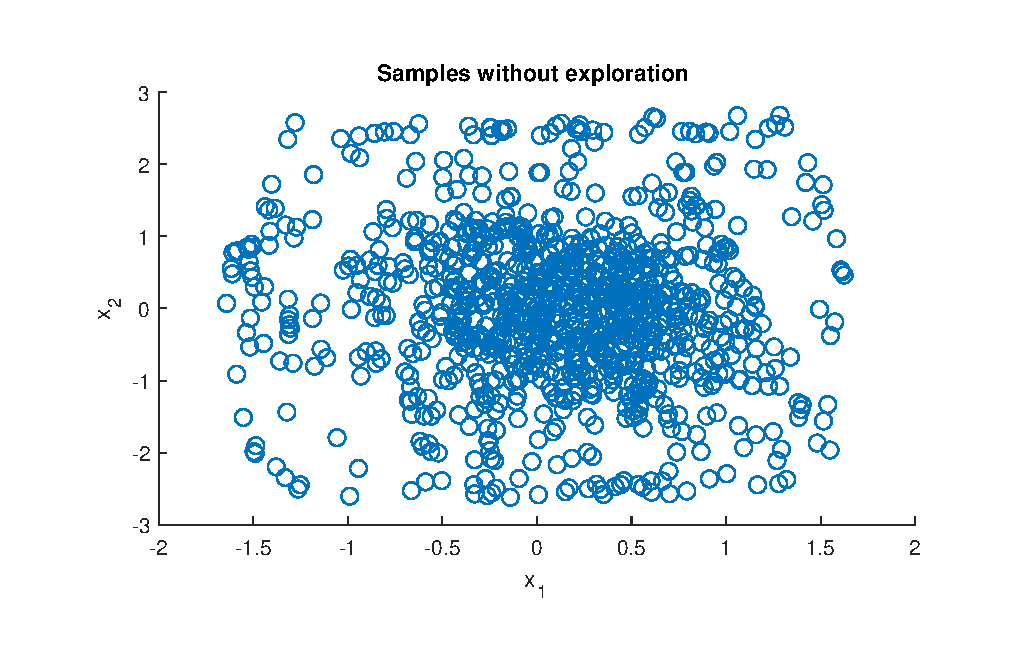
\includegraphics[width=0.7\textwidth]{samples_unexploration}
    \end{subfigure}
    
    \begin{subfigure}[b]{\textwidth}
    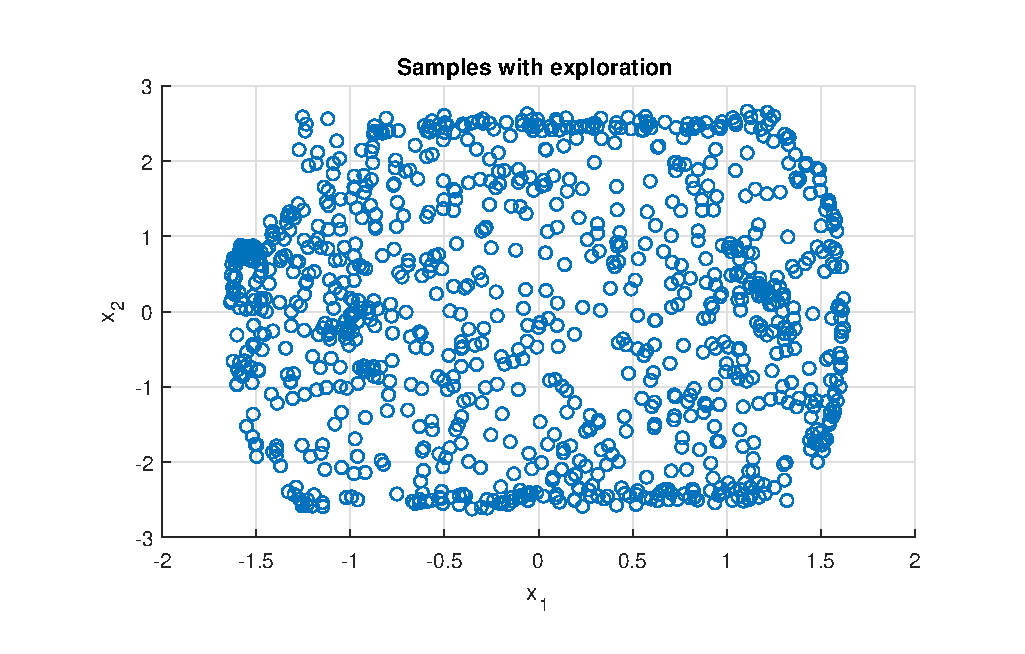
\includegraphics[width=0.7\textwidth]{samples_exploration}
    \end{subfigure}
        \caption{Realisation of samples with and without Incremental Q-learning. In the lower figure, the spread of the samples is clearly better, whereas in the upper figure most samples are concentrated around the origin.}  \label{fig:samples_exploration}
\end{figure}

It is therefore interesting to examine whether the Incremental Q-learning, as described in Section \ref{sec:Exploration}, yields a better estimation of the policy. The results of this comparison are depicted in Figure \ref{fig:policy_exploration}. The figure shows the estimated policy at each state, where the respective colors correspond to values of $u$. The quality of the estimated policy can be decided upon by comparing to the optimal policy which has been found with Policy Iteration (left figure). Clearly, the results are better for the approach which incorporates exploration (middle figure). This can especially be seen at the edges of the safe set, where the estimated policy without exploration is very inaccurate (right figure).

\begin{figure}[H]
    \centering
    \makebox[\textwidth][c]{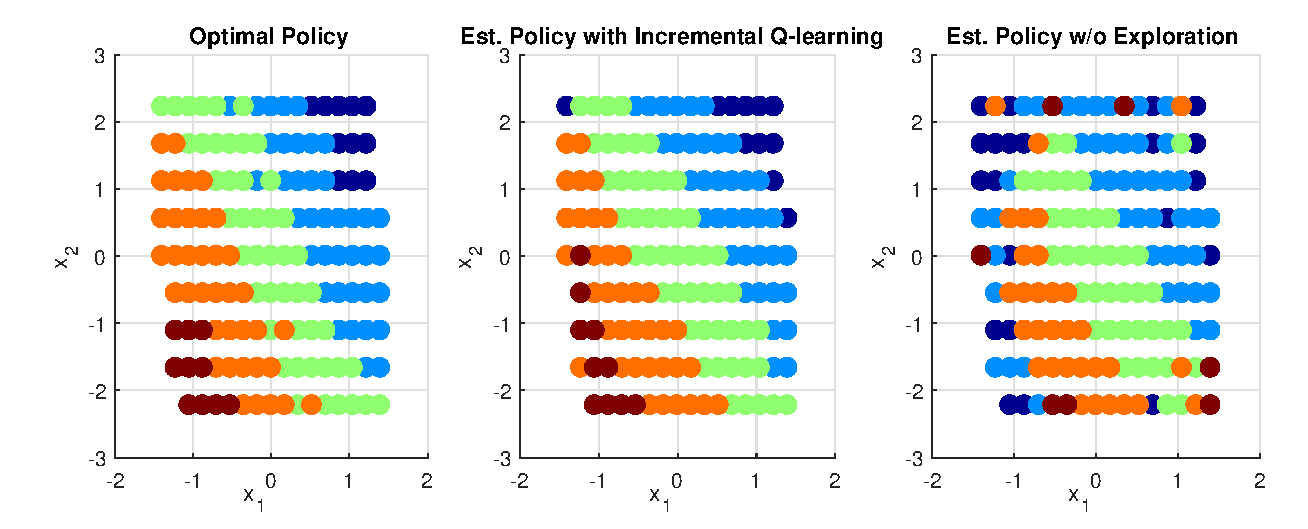
\includegraphics[width=1.2\textwidth]{policy_exploration}}
    \caption{Policy estimated with Incremental Q-learning, $\epsilon$-greedy exploration and without exploration. After the same number of learning iterations, the algorithm with Incremental Q-learning achieves considerably better results above all at the edges of the safe set.} \label{fig:policy_exploration}
\end{figure}

To quantify the findings from Figure \ref{fig:policy_exploration}, the absolute error between the estimated and the optimal policy is illustrated in Figure \ref{fig:PolicyError}. In addition to the algorithm without exploration and with Incremental Q-learning, the error with $\epsilon$-greedy exploration is shown. It becomes apparent that the Incremental Q-learning approach takes slightly longer to converge but ends up with a remarkably better result. One can further conclude that the deterministic approach to exploration, Incremental Q-learning, pays off in comparison to the randomised $\epsilon$-greedy exploration. 

\begin{figure}[H]
    \centering
    \makebox[\textwidth][c]{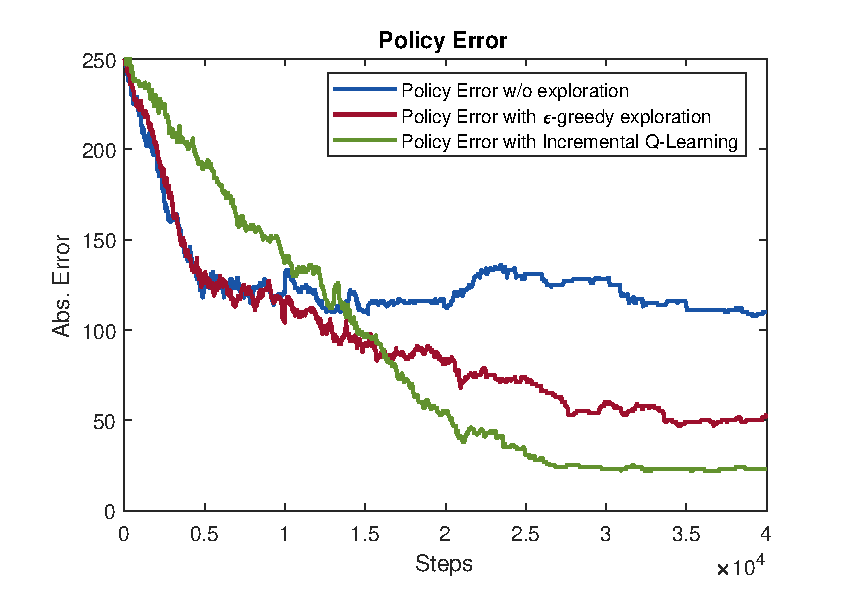
\includegraphics[width=\textwidth]{PolicyError}}
    \caption{Policy error with Incremental Q-learning, $\epsilon$-greedy eploration and without exploration. The approach with Incremental Q-learning converges slightly slower but the final error without exploration is about four times higher than the error of the Incremental Q-learning algorithm.} \label{fig:PolicyError}
\end{figure}

However, in the long run, pure exploration might not be the most desirable strategy. After all states have been visited sufficiently often, one would wish to exploit the most promising strategy. In the present system, this means that after sufficient exploration one would wish to keep the pendulum stable around the origin. This can for example be realised by switching off the exploration after all states have been visited $100$ times. It is therefore interesting to investigate, if the exploration algorithm can guarantee that all states are visited a sufficient number of times. Figure \ref{fig:leastvisited} shows the number of visits of the 10 least visited states with and without exploration. 
\begin{figure}[H]
    \centering
    \makebox[\textwidth][c]{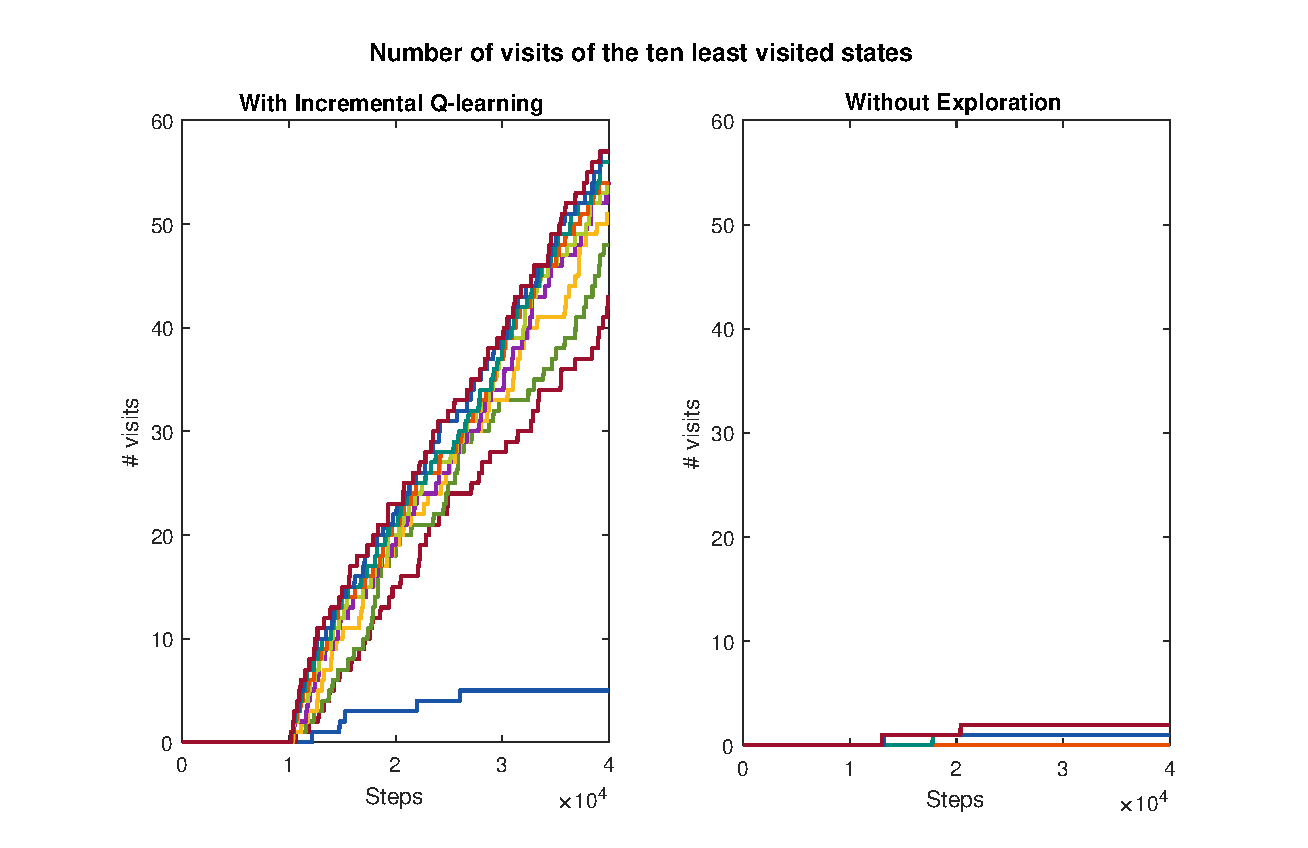
\includegraphics[width=\textwidth]{leastvisited}}
        \caption{Number of visits of the 10 least visited states with and without exploration respectively.}  \label{fig:leastvisited}
\end{figure}
Without exploration, several states remain unvisited for all $40,000$ steps. None of the 10 least visited states is visited more than five times. With Incremental Q-learning, the system samples all states within the first $20,000$ steps. Except from one, all states count more than $40$ visits within the observed $40,000$ steps. This indicates that it might indeed be possible to switch off the Incremental Q-learning after a certain number of iterations. A suitable criterion could be identified by examining how often a state approximately needs to be visited to eliminate the policy error. We stress that in the existing literature, the topic of policy convergence has not yet been well covered as current results mostly focus on the convergence results of state values. \par
\section{Disturbance Estimation and Safe Set Computations}
In this section, the influence of exploration on the disturbance estimation will be examined. Figure \ref{fig:GP_it4_doubleexplore} shows the result from the disturbance estimation with GP regression after each iteration with the setup described above. As only states within the safe set can be visited, no estimate of a policy outside that set can be done. Therefore, only policy values within the safe set are compared. The left and right half of the figure show the result without exploration and Incremental Q-learning, respectively. For both algorithms, it can be seen that the disturbance estimation improves after each iteration. This is due to the fact that the system visits wider regions of the state-space as the number of steps increases. Therefore, the samples taken from the recorded data points are spread out wider as more steps are recorded. Furthermore, it becomes evident that the disturbance estimation indeed is better for the approach with exploration. In the case without exploration, the samples are more concentrated in the front half of the coordinate system so that the disturbance estimate is good in that region but almost constant in the rear half and outside the safe set. In the case with exploration, the sinusoidal shape of the disturbance is clearly visible from the third iteration onwards. The disturbance estimate is quite accurate for all states within the safe set. 

\begin{figure}[H]
    \centering
    \makebox[\textwidth][c]{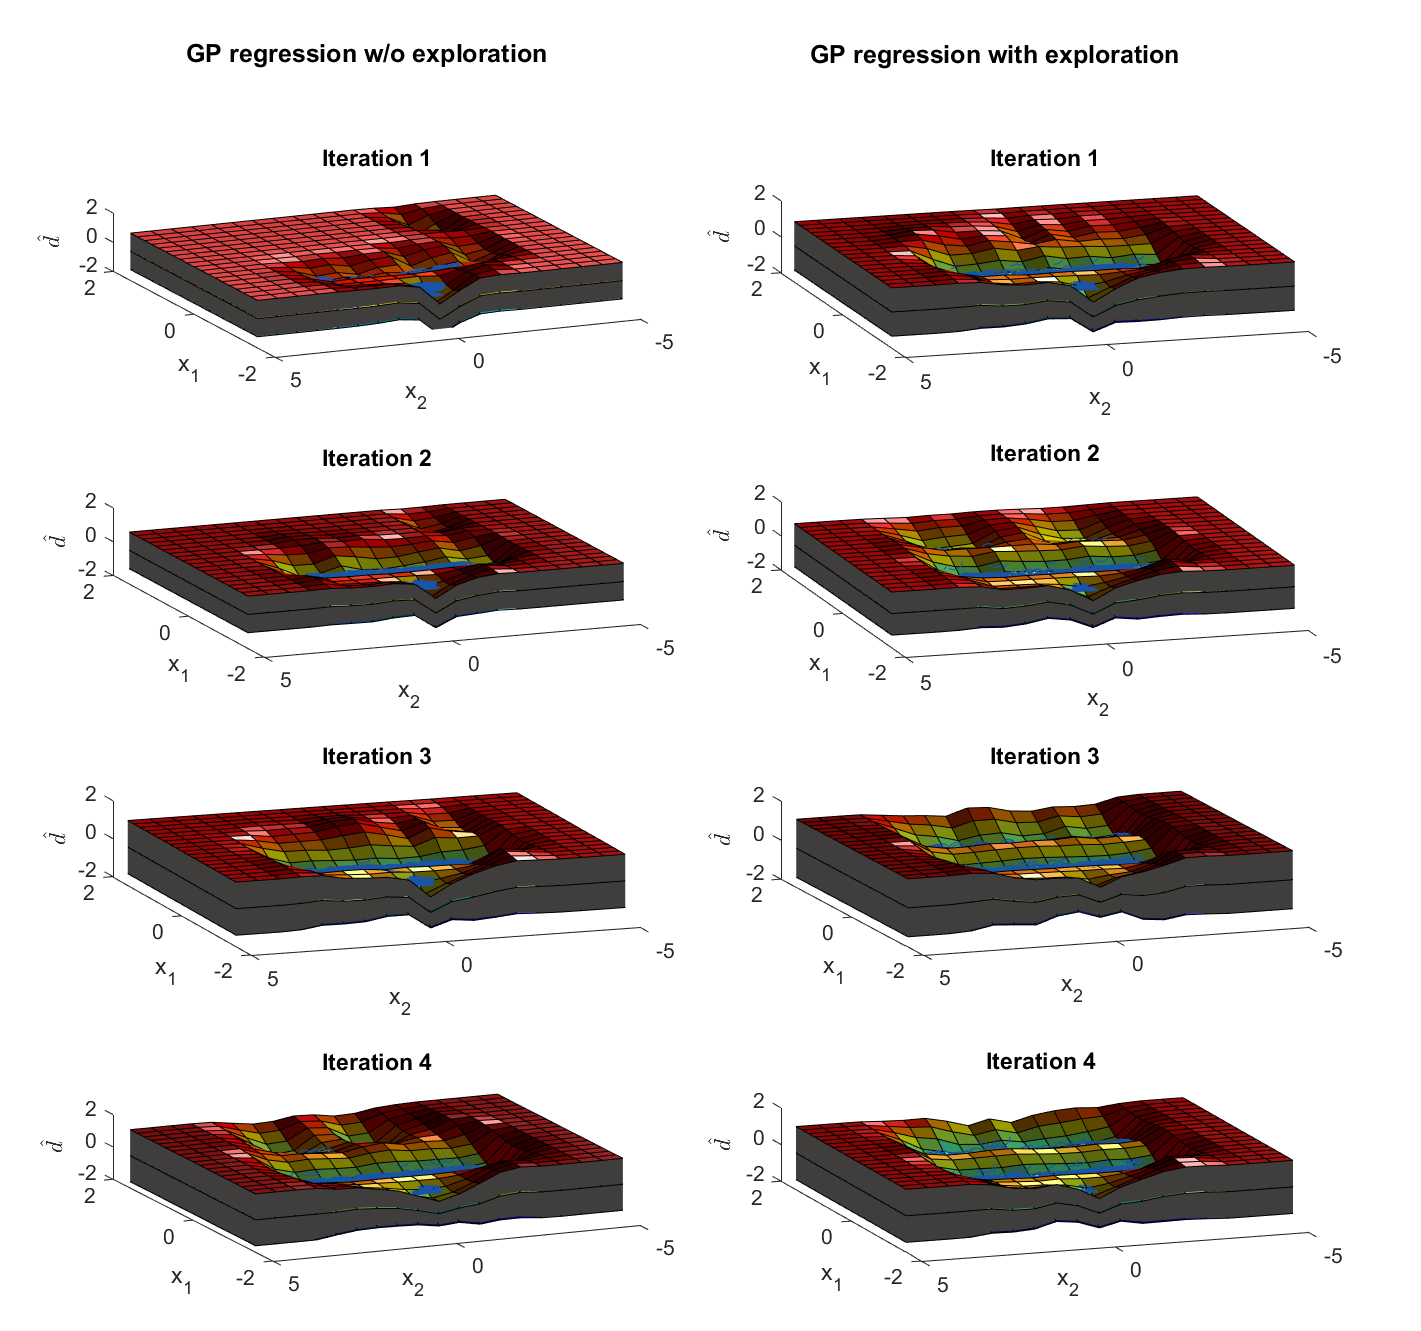
\includegraphics[width=1.2\textwidth]{GP_it4_doubleexplore}}
        \caption{GP regression in four iterations with each 10,000 steps.}  \label{fig:GP_it4_doubleexplore}
\end{figure}


Figure \ref{fig:SafeSet_it4_unexplore} shows the safe set computations for all four iterations. During the first iteration, the conservative initial range is used for the safe set calculations and gives a relatively small initial safe set. By calculating a better disturbance estimate in the GP regression, the safe set grows already largely in the second iteration. 
\begin{figure}[H]
    \centering
    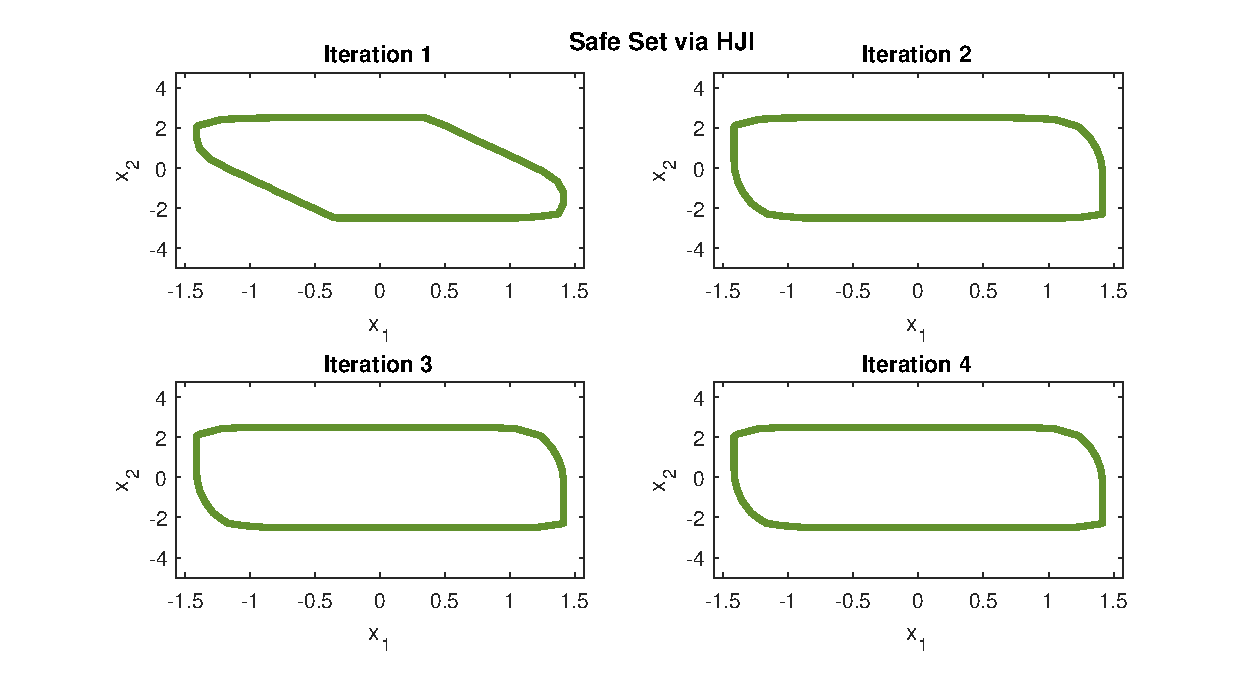
\includegraphics[width=\textwidth]{SafeSet_it4_unexplore}
        \caption{The evolution of the safe set in four iterations. The better disturbance estimate causes a lare increase of the safe set in the second iteration.}  \label{fig:SafeSet_it4_unexplore}
\end{figure}

Interestingly, the safe set resulting from the disturbance estimate is the same without and with exploration. This could be attributed to the fact that the safe set is an over-approximation of the true safe set that not necessarily increases as the disturbance bounds decrease. This claim is supported by the fact that the safe set remains the same even if a disturbance of $d = 0\,\text{N}$ is assumed.\par
\section{System Trajectories in State-Space and Time Representation}
Finally, simulation results from both approaches are portrayed in Figure \ref{fig:Simulation}. The depicted trajectories show the last $500,000$ samples of the test run with four iterations that have been recorded with $h_\text{safe} = 0.005\,\text{s}$. It becomes clear that the algorithm with exploration causes the system to explore the whole state-space and repeatedly hits the borders of the safe set. Since the safety check is not performed continuously, the system leaves the safe set at some points, but can each time be brought back into the set. In the right half of the figure, it is apparent that the approach without exploration manages to keep the system close to the origin. \par
In a conclusion, it can be said that the presented approach manages to safely learn a control. Our results show that explicit exploration indeed leads to significant better learning results at the edges of the safe set. However, it is still an open question when to shut off the exploration.

\begin{figure}
    \centering
    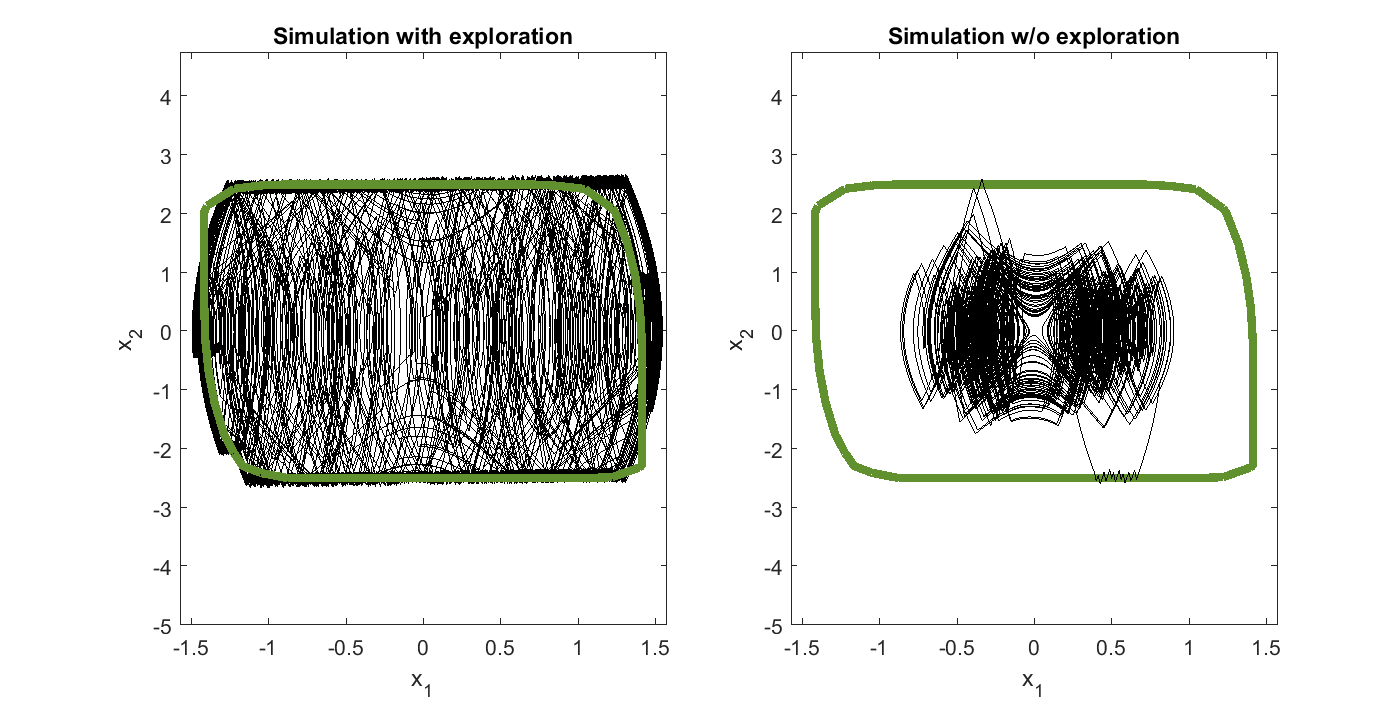
\includegraphics[width=\textwidth]{Simulation}
        \caption{Simulation of the system with Incremental Q-learning versus simulation without exploration. The figure shows the last $500,000$ samples of the test run in state-space.}\label{fig:Simulation}
\end{figure}

To illustrate the whole learning process over time, simulation results with and without exploration are shown in \ref{fig:Simulation_time}. With exploration, the controller keeps exploring the borders of the safe set. Without exploration, the controller keeps the system closer to the origin after a policy has been learned. During the last 1500 seconds, the system never hits the borders of the safe set.

\begin{figure}
    \centering
    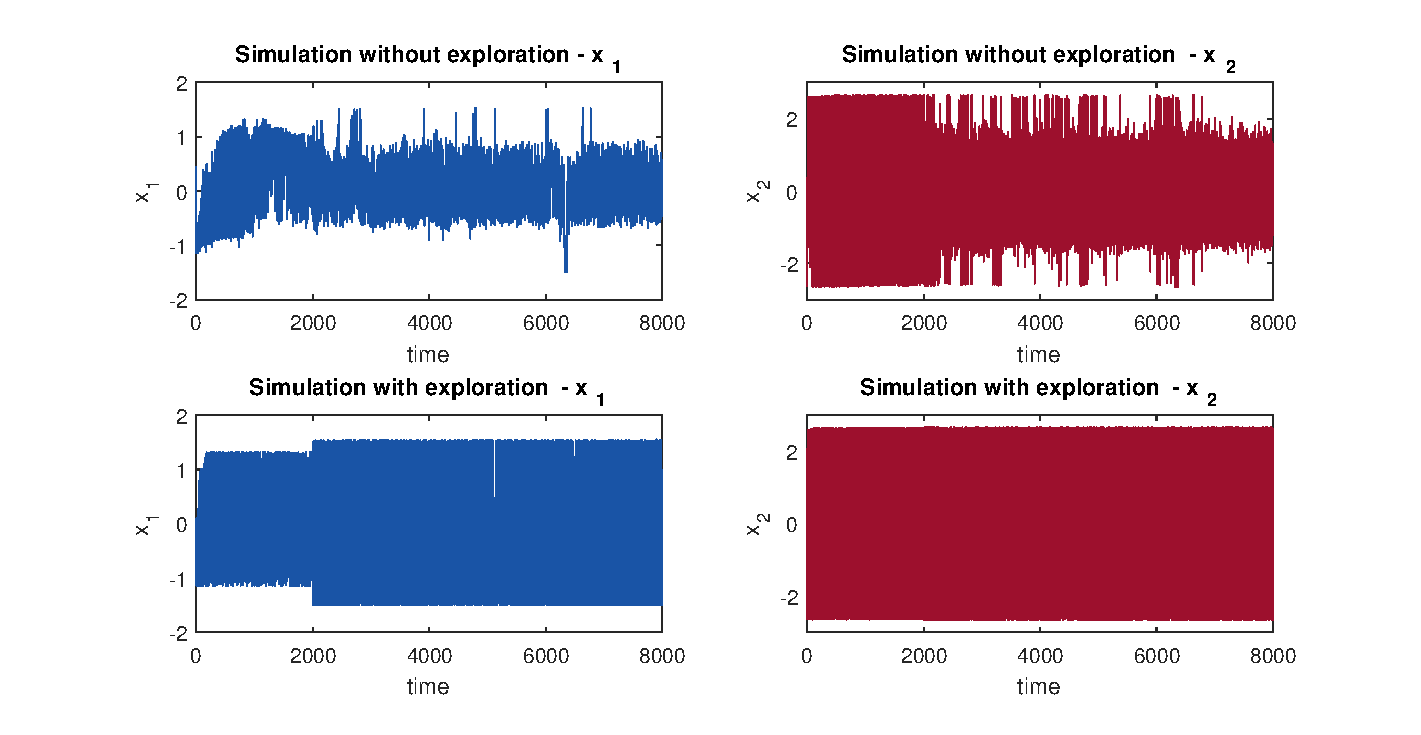
\includegraphics[width=\textwidth]{Simulation_time}
        \caption{Simulation of the system with Incremental Q-learning versus simulation without exploration. The figure shows the whole learning process over time (in seconds).}\label{fig:Simulation_time}
\end{figure}
Further simulations have been conducted, following the idea that exploration should be shut off after a sufficiently good policy has been learned everywhere in the state-space. To this end, exploration was shut off after three iterations and the results of the fourth iteration have been compared to the fourth iteration of a run completely without exploration. To examine if the approach with exploration in the beginning yields better results, difficult initial conditions (i.e. close to the border of the safe set) have been chosen. Two exemplary initial conditions are portrayed in \ref{fig:Simulation_shutoff}. In both images, it can be seen that the system is stabilised quicker (a larger part of the trajectory lies close to the equlibrium point) if exploration has been done during the first iterations. However, the decision when to switch off exploration was purely based on earlier experience with the present system and should be systematised.

\begin{figure}[H]
    \centering
    \begin{subfigure}[b]{\textwidth}
    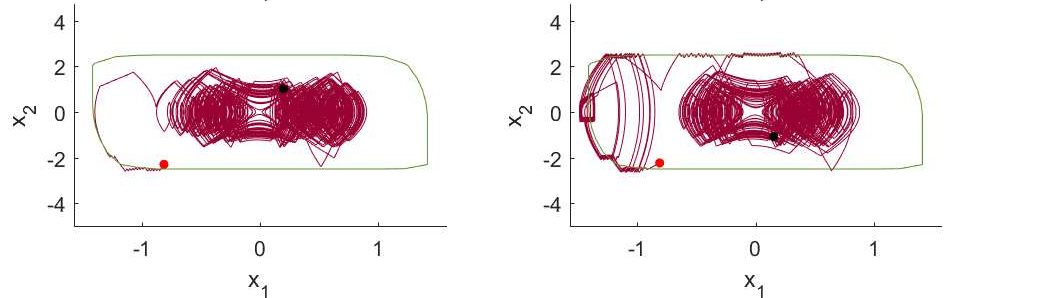
\includegraphics[width=\textwidth]{switch_lower}
    \end{subfigure}
    
    \begin{subfigure}[b]{\textwidth}
    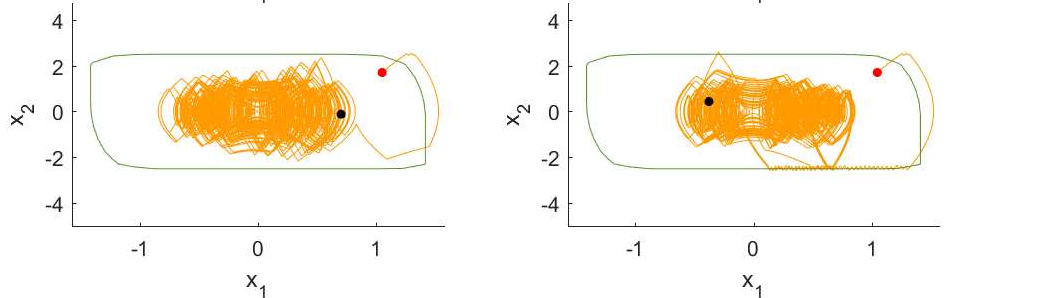
\includegraphics[width=\textwidth]{switch_middle}
    \end{subfigure}
        \caption{Comparison of system trajectories during the fourth (exploitary) iteration of a test run after three iterations with exploration (left) and three iterations without exploration (right).}  \label{fig:Simulation_shutoff}
\end{figure}


\end{document}
